% ============================================================================
% IEEE Conference Paper: Boundary-Local Rank Redundancy in Selective Prediction
% Target: IEEE India Conference (6 pages), Overleaf-ready
% Single-focus revision: the paper's one contribution is the rho_local
% diagnostic (theorem + empirical validation + practical protocol) and the
% benchmarking-bias finding that motivates needing it. Everything not in
% direct service of that claim (conformal risk control, subgroup fairness,
% the coverage-targeted-loss architecture) is compressed to a sentence or
% moved out, so a reviewer is never asked to read machinery the paper's own
% conclusion does not depend on.
% ============================================================================
\documentclass[conference]{IEEEtran}

% --- Packages ---
\usepackage{cite}
\usepackage{amsmath,amssymb,amsfonts}
\usepackage{graphicx}
\usepackage{booktabs}
\usepackage{multirow}
\usepackage{xcolor}
\usepackage{algorithm}
\usepackage{algorithmic}
\usepackage{url}
\usepackage{textcomp}

% --- Graphics Path ---
\graphicspath{{figures/}}

% --- Custom Commands ---
\newcommand{\aurc}{\mathrm{AURC}}
\newcommand{\rholocal}{\rho_{\mathrm{local}}}
\newcommand{\rhoglobal}{\rho_{\mathrm{global}}}

\begin{document}

% ============================================================================
% TITLE & AUTHORS
% ============================================================================
\title{Boundary-Local Rank Redundancy: A Diagnostic for When\\Uncertainty Aggregation Helps Selective Prediction}

\author{
  \IEEEauthorblockN{Samihan Narayankeri}
  \IEEEauthorblockA{Dept.\ of AI \& DS\\
    BRACT's Vishwakarma Institute\\of Information Technology\\
    Savitribai Phule Pune University\\
    Pune, India\\
    samihan.22311426@viit.ac.in}
  \and
  \IEEEauthorblockN{Yash Kale}
  \IEEEauthorblockA{Dept.\ of AI \& DS\\
    BRACT's Vishwakarma Institute\\of Information Technology\\
    Savitribai Phule Pune University\\
    Pune, India\\
    yash.kale@viit.ac.in}
  \and
  \IEEEauthorblockN{Yash Swami}
  \IEEEauthorblockA{Dept.\ of AI \& DS\\
    BRACT's Vishwakarma Institute\\of Information Technology\\
    Savitribai Phule Pune University\\
    Pune, India\\
    yash.swami@viit.ac.in}
  \and
  \IEEEauthorblockN{Tanishka Nagawade}
  \IEEEauthorblockA{Dept.\ of AI \& DS\\
    BRACT's Vishwakarma Institute\\of Information Technology\\
    Savitribai Phule Pune University\\
    Pune, India\\
    tanishka.nagawade@viit.ac.in}
  \and
  \IEEEauthorblockN{Amar Buchade}
  \IEEEauthorblockA{Associate Professor\\
    Dept.\ of AI \& DS\\
    BRACT's Vishwakarma Institute\\of Technology\\
    Savitribai Phule Pune University\\
    Pune, India\\
    amar.buchade@vit.edu}
}

\maketitle

% ============================================================================
% ABSTRACT
% ============================================================================
\begin{abstract}
Selective classifiers abstain on inputs they are unlikely to classify correctly, trading coverage for reliability. A common design pattern aggregates a heterogeneous bank of uncertainty signals -- calibrated confidence, ensemble disagreement, energy scores, feature-space geometry -- hoping their combination outranks the best individual signal. We show this hope is often false for a provable, structural reason, and we give practitioners a cheap, label-free diagnostic that predicts in advance whether it is false for a given signal bank and dataset.

On binary classification tasks, every logit-derived confidence signal is a strictly monotone transform of the same scalar margin ($|\rho_{\mathrm{Spearman}}| = 1.0000$ across three datasets, confirmed exactly across 48 base-model-capacity settings with zero exceptions), so no aggregator over such a bank can ever outrank maximum softmax probability (MSP). The area under the risk--coverage curve (AURC) depends only on this ranking, and it is dominated by the ordering of points near the abstention boundary, not by the whole test set -- so redundancy must be measured there. We introduce \emph{boundary-local rank redundancy} ($\rholocal$), the minimum pairwise rank correlation among a signal bank restricted to the top-$q$ riskiest points, and show it separates six benchmark datasets by aggregation outcome with zero overlap across seeds, while the conventional \emph{global} correlation is blind to the same effect on two of those six datasets. We further show that typical tabular selective-prediction benchmarks are statistically under-powered to detect the modest effects aggregation does produce, which is exactly the condition under which a label-free, pre-deployment screening rule is most valuable. We package $\rholocal$ as a three-line protocol a practitioner can run on unlabelled held-out data before ever training an aggregator, and report honestly where our own attempt to establish its causal status (rather than its predictive one) at fixed class count did not succeed.
\end{abstract}

\begin{IEEEkeywords}
selective classification, uncertainty quantification, rank aggregation, abstention, benchmark evaluation, AURC, tabular data
\end{IEEEkeywords}

% ============================================================================
% I. INTRODUCTION
% ============================================================================
\section{Introduction}
\label{sec:intro}

Deploying machine learning in safety-critical domains -- healthcare, finance, autonomous systems -- demands that models recognize when they are likely to err and abstain rather than guess. Chow's rule~\cite{chow1970}, which abstains when the maximum predicted posterior falls below a threshold, is Bayes-optimal \emph{given correct posteriors}. In practice, modern classifiers are miscalibrated~\cite{guo2017calibration}, behave unpredictably on out-of-distribution inputs~\cite{liu2020energy}, and carry epistemic uncertainty invisible to a single forward pass. A comprehensive benchmark of 18 selective-classification methods across 44 datasets found that no single method dominates~\cite{pugnana2024benchmark}, which motivates combining several uncertainty signals into one aggregated score rather than trusting any one of them.

Yet a well-tuned MSP baseline is a notoriously strong competitor. Feng et al.~\cite{feng2023better} showed that elaborate learned-abstention methods often fail to beat it, and Cattelan and Silva~\cite{cattelan2023logitnorm} demonstrated that cheap post-hoc fixes recover much of the claimed gain of heavier methods. These are consistent, repeated observations across independent studies, and they call for a mechanism, not another benchmark entry. This paper supplies one: we prove that on binary tasks, a large and commonly-used family of confidence signals is \emph{exactly rank-degenerate}, so aggregation cannot possibly help -- and we generalize the diagnosis into a practical tool, $\rholocal$, that predicts when the same failure mode occurs on multiclass problems where the degeneracy is not exact.

\textbf{Contribution.} We contribute one diagnostic, in three parts, and report the evidence for and against each part with equal weight:
\begin{enumerate}
  \item \textbf{A proof} that logit-derived signals are rank-degenerate on binary tasks ($|\rho|{=}1.0000$ across three datasets, and across every one of 48 base-model-capacity settings we tested), which bounds what \emph{any} aggregator over such a bank can achieve.
  \item \textbf{A boundary-local redundancy diagnostic} ($\rholocal$), computable on unlabelled held-out data before an aggregator is ever trained, that predicts the aggregation outcome on 6/6 benchmark datasets with zero seed overlap -- where the conventional global correlation is blind to the same effect.
  \item \textbf{An honest account of what the diagnostic is not yet}: an error-count power analysis showing why the benchmarking evidence for aggregation is generally too weak to resolve on its own, and a controlled experiment in which our attempt to establish $\rholocal$ as \emph{causal} (rather than merely predictive) at fixed class count produced a genuine negative result on one dataset and no dose-response on another.
\end{enumerate}

% ============================================================================
% II. RELATED WORK
% ============================================================================
\section{Related Work}
\label{sec:related}

\textbf{Foundations.} Chow~\cite{chow1970} established the optimal reject rule. El-Yaniv and Wiener~\cite{elyaniv2010foundations} formalized the risk--coverage trade-off, and Geifman and El-Yaniv~\cite{geifman2017selective} established the evaluation protocol we follow. Our binary-degeneracy result identifies a regime where Chow's rule is not merely strong but \emph{unimprovable} by any logit-derived competitor.

\textbf{Learned Abstention.} SelectiveNet~\cite{geifman2019selectivenet} adds a selection head; Deep Gamblers~\cite{liu2019deepgamblers} recasts abstention as an extra class; ConfidNet~\cite{corbiere2019confidnet} learns true-class probability; CRL~\cite{moon2020crl} regularizes confidence ranking; and learning-to-defer~\cite{mozannar2020defer} targets the human-in-the-loop variant. All require retraining the base model; the aggregation approach we analyze is strictly post-hoc, and is the more common pattern where retraining is infeasible.

\textbf{Strong Baselines.} Feng et al.~\cite{feng2023better} argue a tuned softmax baseline matches elaborate methods; Cattelan and Silva~\cite{cattelan2023logitnorm} show cheap post-hoc repairs recover much of the claimed gain of heavier methods, and note that logit normalization is degenerate at $K{=}2$ -- a limitation of the published method our own binary-degeneracy result generalizes to an entire signal family.

\textbf{Signal Sources.} Our bank draws on temperature scaling~\cite{guo2017calibration}, deep ensembles~\cite{lakshminarayanan2017ensembles}, the energy score~\cite{liu2020energy}, Mahalanobis distance~\cite{lee2018mahalanobis}, $k$-NN distance~\cite{sun2022knn}, and trust score~\cite{jiang2018trustscore}.

\textbf{Scope note.} Our post-hoc scores can additionally be wrapped in a distribution-free risk-control guarantee~\cite{angelopoulos2022riskcontrol,angelopoulos2021learnthentest}, and selective classification is known to widen subgroup disparities~\cite{jones2021disparities}; both are part of the broader system this bank was built for, but neither bears on the redundancy question this paper is about, so we do not report results on them here.

% ============================================================================
% III. PRELIMINARIES
% ============================================================================
\section{Preliminaries}
\label{sec:prelim}

Let $f$ be a frozen $K$-class classifier and $g: \mathcal{X} \to \{0,1\}$ a selection function. \textbf{Coverage} is $\Phi(g) = \Pr[g(x)=1]$. \textbf{Selective risk} is
\begin{equation}
  R(f,g) = \frac{\mathbb{E}[\ell(f(x),y) \cdot g(x)]}{\mathbb{E}[g(x)]},
\end{equation}
where $\ell$ is 0--1 loss. The \textbf{risk--coverage curve} plots $R(f, g_\tau)$ against $\Phi(g_\tau)$ as a threshold $\tau$ on score $s(x)$ varies. $\aurc$ (Area Under the Risk-Coverage curve, lower is better) is its integral.

\textbf{The property that makes the diagnostic possible.} $\aurc$ depends only on the \emph{ranking} $s$ induces on the test set -- two scores with the same ranking give identical $\aurc$. Three consequences follow, and the third is the one prior redundancy analyses miss. (i) Only ordinal information matters, so any monotone reparameterization of a signal is free. (ii) At prefix length $k$, $\aurc$'s cumulative error rate has denominator $k$, so a rank swap near $k{=}3$ moves the curve by $O(1/3)$ while one near $k{=}3000$ moves it by $O(1/3000)$: $\aurc$ is dominated by the ordering of the points most likely to be abstained on, not by the test set as a whole. (iii) Calibration is irrelevant to $\aurc$, since it is invariant to any order-preserving rescaling.

% ============================================================================
% IV. METHOD
% ============================================================================
\section{Method}
\label{sec:method}

\subsection{Signal Bank}
Given input $x$ and frozen base model $f$, we compute $u(x) \in \mathbb{R}^m$ from three tiers. \textbf{Tier A (logit-derived):} MSP ($1{-}\max_k p_k$), predictive entropy, probability margin, logit margin, an energy score (mean-centered for correctness at $K{=}2$), temperature-scaled MSP, and a calibration residual. \textbf{Tier B (ensemble):} vote entropy, mean pairwise KL divergence, and top-class variance from a 5-member ensemble. \textbf{Tier C (geometry):} $k$-NN distance, local label agreement, trust score~\cite{jiang2018trustscore}, and Mahalanobis distance to the predicted-class centroid~\cite{lee2018mahalanobis}. Tier A is where the degeneracy theorem in \S\ref{sec:degeneracy} applies exactly, and it is the sub-bank $\rholocal$ is defined over.

\subsection{Aggregators}
We evaluate a parameter-free rank/z-score average (A0), logistic-regression or LightGBM stacking on correctness (A1), and an MLP trained with coverage-targeted losses plus an instance-adaptive gating variant (A2). A2's architecture and losses are not this paper's subject; \S\ref{sec:ablations} reports only the one fact about it that bears on our claim -- it never outperforms the simpler alternatives, so aggregator sophistication is not the axis this paper's finding lives on.

% ============================================================================
% V. EXPERIMENTAL SETUP
% ============================================================================
\section{Experimental Setup}
\label{sec:setup}

\textbf{Datasets.} Six OpenML datasets, screened on \emph{test-error count} rather than row count (\S\ref{sec:limitations} explains why): three binary -- Adult ($n_{\mathrm{err}}{=}944$), German Credit ($n_{\mathrm{err}}{=}34$), Electricity (temporal shift, $n_{\mathrm{err}}{=}2{,}533$) -- and three multiclass -- Satimage ($K{=}6$, $n_{\mathrm{err}}{=}67$), Wine Quality ($K{=}7$, $n_{\mathrm{err}}{=}236$), Letter ($K{=}26$, $n_{\mathrm{err}}{=}82$). Four candidates with fewer than 12 test errors were rejected before being admitted.

\textbf{Protocol.} Disjoint four-way split ($D_{\mathrm{train}}$ 60\%, $D_{\mathrm{meta}}$ 15\%, $D_{\mathrm{cal}}$ 10\%, $D_{\mathrm{test}}$ 15\%). Signals are computed via 5-fold cross-fitting over $D_{\mathrm{train}} \cup D_{\mathrm{meta}}$ to prevent leakage into aggregator training. Base model: LightGBM (300 trees, row/column subsampling so each of 10 seeds trains a genuinely different model). All results use 10 seeds unless noted.

\textbf{Metrics.} $\aurc$ (primary). Significance: paired Wilcoxon signed-rank with Holm--Bonferroni correction, and a paired per-instance bootstrap (\S\ref{sec:power}).

% ============================================================================
% VI. RESULTS
% ============================================================================
\section{Results}
\label{sec:results}

\subsection{Tier-A Signals Are Rank-Degenerate on Binary Tasks}
\label{sec:degeneracy}

At $K{=}2$, a softmax reads only the single scalar logit difference $s$. MSP, entropy, both margins, temperature-scaled MSP, and centered energy are therefore strictly monotone transforms of one another. Because $\aurc$ depends only on the induced ordering, all produce \emph{identical} risk--coverage curves. Measured $|\rho_{\mathrm{Spearman}}|$ against MSP is $1.0000$ for all comparators on all three binary datasets across 10 seeds. We additionally confirm this holds independent of base-model capacity: across 48 (dataset, seed, capacity) combinations spanning a 3-tree model trained on 2\% of the data up to the full 300-tree model, $\rholocal$ never departed from $1.0000$ by more than $10^{-6}$. The consequence: on a binary task, a bank of six Tier-A signals contains exactly \emph{one} ranking, and no aggregator can improve on MSP, however it is trained.

At $K \ge 3$, the degeneracy partially breaks (energy decorrelates to $0.96$ on Satimage, $0.71$ on Wine), but unevenly: entropy remains at $1.0000$ against MSP on Satimage. Multiclass structure is sufficient to break the degeneracy but does not by itself guarantee a diverse bank.

\begin{figure*}[t]
\centering
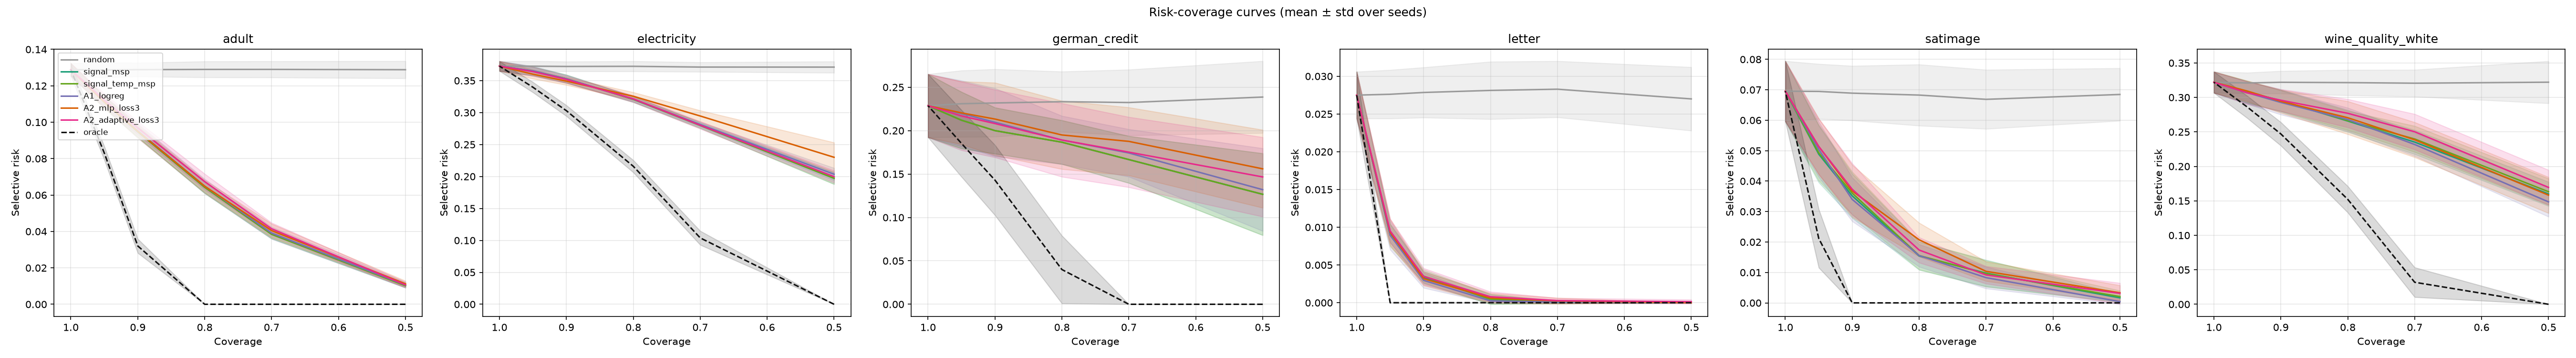
\includegraphics[width=0.95\textwidth]{figures/risk_coverage_curves.png}
\caption{Selective risk versus coverage across all six datasets (10 seeds, LightGBM base classifier). Aggregation yields visible improvements primarily on multiclass benchmarks (Satimage, Letter), while matching or trailing MSP on binary tasks -- exactly as the degeneracy result predicts.}
\label{fig:risk_coverage}
\end{figure*}

\begin{table*}[t]
\centering
\caption{$\aurc$ (lower is better), mean over 10 seeds, signal tiers A+C. $\dagger$ = temporal-shift split.}
\label{tab:main_aurc}
\begin{tabular}{l r rrrrrrrr}
\toprule
Dataset & $K$ & MSP & A0\_rank & A1\_logreg & A2\_mlp\_bce & A2\_mlp\_loss3 & A2\_adaptive & oracle & random \\
\midrule
Adult & 2 & 0.0302 & 0.0331 & 0.0304 & 0.0309 & 0.0310 & 0.0320 & 0.0087 & 0.1284 \\
Electricity$^{\dagger}$ & 2 & 0.1946 & 0.1969 & 0.1997 & 0.2119 & 0.2292 & 0.1953 & 0.0802 & 0.3705 \\
German Credit & 2 & 0.1330 & 0.1248 & 0.1341 & 0.1528 & 0.1484 & 0.1469 & 0.0299 & 0.2465 \\
Satimage & 6 & 0.0100 & 0.0102 & \textbf{0.0093} & 0.0110 & 0.0115 & 0.0106 & 0.0026 & 0.0697 \\
Wine Quality & 7 & 0.1846 & 0.1648 & \textbf{0.1394} & 0.1486 & 0.1463 & 0.1548 & 0.0589 & 0.3202 \\
Letter & 26 & 0.0013 & 0.0015 & \textbf{0.0012} & 0.0013 & 0.0013 & 0.0014 & 0.0004 & 0.0266 \\
\bottomrule
\end{tabular}
\end{table*}

\begin{table}[t]
\centering
\caption{Aggregation vs.\ the best single signal (best-of-$N$ over 9 aggregators and up to 12 signals). Negative $\Delta$ favours aggregation. German Credit's $-6.2\%$ is a selection artefact: pre-registering \texttt{A1\_logreg} in advance flips it to $+2.9\%$ (\S\ref{sec:power}).}
\label{tab:agg_vs_single}
\begin{tabular}{l r l r r}
\toprule
Dataset & $K$ & Best single & Best agg. & $\Delta$ \\
\midrule
Adult & 2 & energy\,(0.030) & 0.030 & +0.9\% \\
Electricity$^{\dagger}$ & 2 & energy\,(0.195) & 0.195 & +0.4\% \\
German Credit & 2 & energy\,(0.133) & 0.125 & -6.2\% \\
Satimage & 6 & entropy\,(0.010) & 0.009 & \textbf{-6.4\%} \\
Wine Quality & 7 & trust\,(0.141) & 0.139 & -1.3\% \\
Letter & 26 & entropy\,(0.001) & 0.001 & \textbf{-6.3\%} \\
\bottomrule
\end{tabular}
\end{table}

\subsection{Boundary-Local Redundancy Predicts Aggregation Outcome}
\label{sec:mechanism}

Since $\aurc$ weights a rank swap at prefix $k$ by $O(1/k)$ (\S\ref{sec:prelim}), redundancy should be measured \emph{where $\aurc$ is sensitive} -- the abstention candidates -- not over the whole test set. We define
\begin{equation}
  \rholocal(q) = \min_{j \in \mathcal{A} \setminus \{\mathrm{ref}\}} \bigl| \rho_{\mathrm{Spearman}}(u_{\mathrm{ref}}, u_j) \bigr| \Big|_{\mathcal{Q}_q},
  \label{eq:rholocal}
\end{equation}
where $\mathcal{Q}_q$ is the top-$q$ fraction of points ranked by the reference signal $u_{\mathrm{ref}}$ (MSP) and $\mathcal{A}$ is the Tier-A sub-bank. If $\rholocal{=}1$, every Tier-A signal induces the same order as MSP where it matters, so the bank carries exactly one ordinal degree of freedom there and no aggregator can exploit it; on a binary task this holds \emph{exactly}, by \S\ref{sec:degeneracy}, at every $q$.

\begin{figure}[t]
\centering
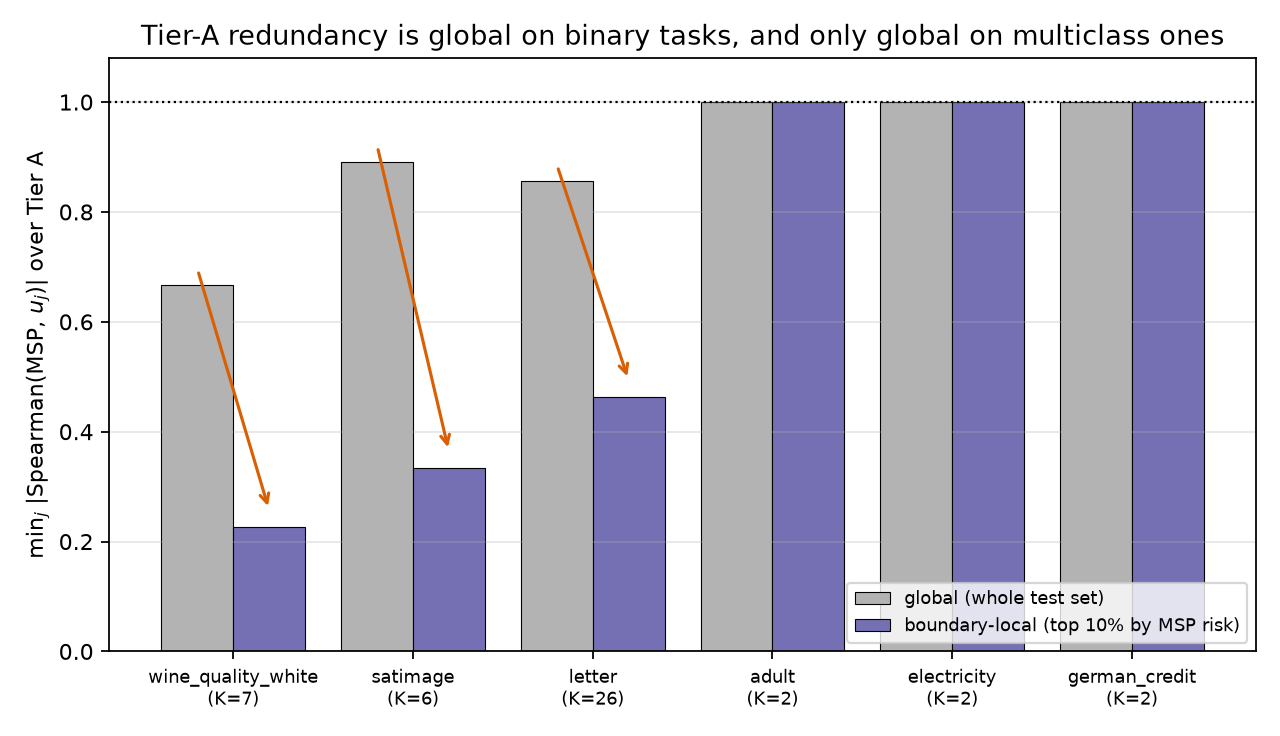
\includegraphics[width=\columnwidth]{figures/redundancy_global_vs_local.png}
\caption{Tier-A redundancy measured globally (grey) versus in the boundary region (purple), $q{=}0.10$. On Satimage and Letter the global statistic reads $0.86$--$0.89$ and would be read as ``redundant''; the same banks decorrelate to $0.33$--$0.46$ exactly where the ranking that determines $\aurc$ is decided.}
\label{fig:global_vs_local}
\end{figure}

Table~\ref{tab:rho_local} and Fig.~\ref{fig:global_vs_local} give both statistics at $q{=}0.10$ against the realized gain of the pre-registered aggregator (\texttt{A1\_logreg}, chosen on the principle that it is the simplest learned method, not on any result). The separation is \textbf{perfect}: $\rholocal{=}1.0000$ on all three datasets where aggregation hurts, $\le 0.46$ on all three where it helps, zero overlap across 60 dataset--seed pairs. The global statistic reads $0.86$--$0.89$ on Satimage and Letter -- falsely suggesting redundancy -- while the local statistic on the same banks reads $0.33$ and $0.46$.

\begin{figure}[t]
\centering
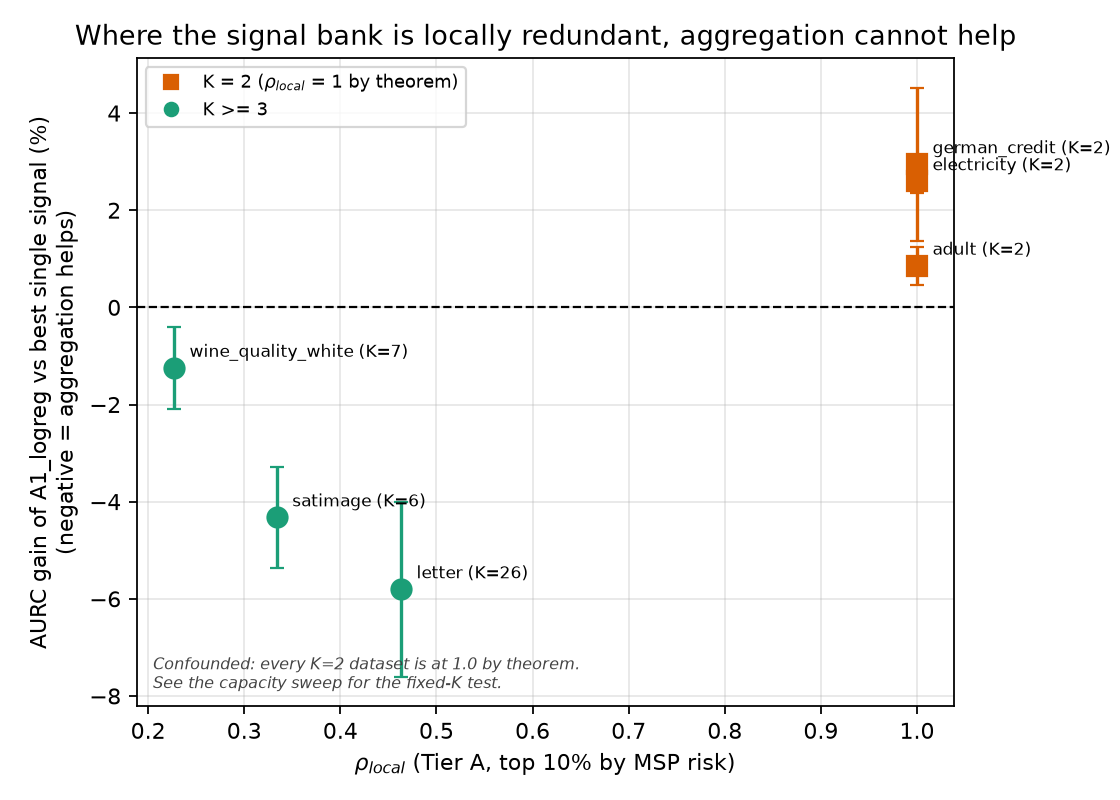
\includegraphics[width=\columnwidth]{figures/rho_local_vs_gain.png}
\caption{Realized $\aurc$ gain of the pre-registered aggregator versus $\rholocal(0.10)$. Binary datasets (squares) sit exactly at $\rholocal{=}1$, as the theorem requires; multiclass datasets (circles) fall below it, with lower $\rholocal$ associated with the datasets where aggregation helps.}
\label{fig:rho_local_gain}
\end{figure}

\begin{table}[t]
\centering
\caption{Boundary-local vs.\ global Tier-A rank redundancy, and the realised $\aurc$ gain of the pre-registered \texttt{A1\_logreg} over the best single signal. Negative $\Delta$ favours aggregation.}
\label{tab:rho_local}
\begin{tabular}{l r r r r}
\toprule
Dataset & $K$ & $\rhoglobal$ & $\rholocal$ & $\Delta\aurc$ \\
\midrule
Adult & 2 & 1.000 & \textbf{1.000} & +0.86\% \\
Electricity$^{\dagger}$ & 2 & 1.000 & \textbf{1.000} & +2.59\% \\
German Credit & 2 & 1.000 & \textbf{1.000} & +2.94\% \\
\midrule
Satimage & 6 & 0.891 & \textbf{0.334} & -4.33\% \\
Wine Quality & 7 & 0.667 & \textbf{0.227} & -1.25\% \\
Letter & 26 & 0.856 & \textbf{0.463} & -5.81\% \\
\bottomrule
\end{tabular}
\end{table}

\subsection{Why Benchmarks Miss This: An AURC Power Analysis}
\label{sec:power}

A risk--coverage curve is built entirely from test-set \emph{errors}, not rows: a 20{,}000-row dataset at 99\% accuracy carries the statistical weight of 200 points, not 20{,}000. This is precisely why a label-free diagnostic like $\rholocal$ is valuable -- it does not need enough errors to resolve an $\aurc$ difference at all, only enough points to estimate a rank correlation.

\begin{figure}[t]
\centering
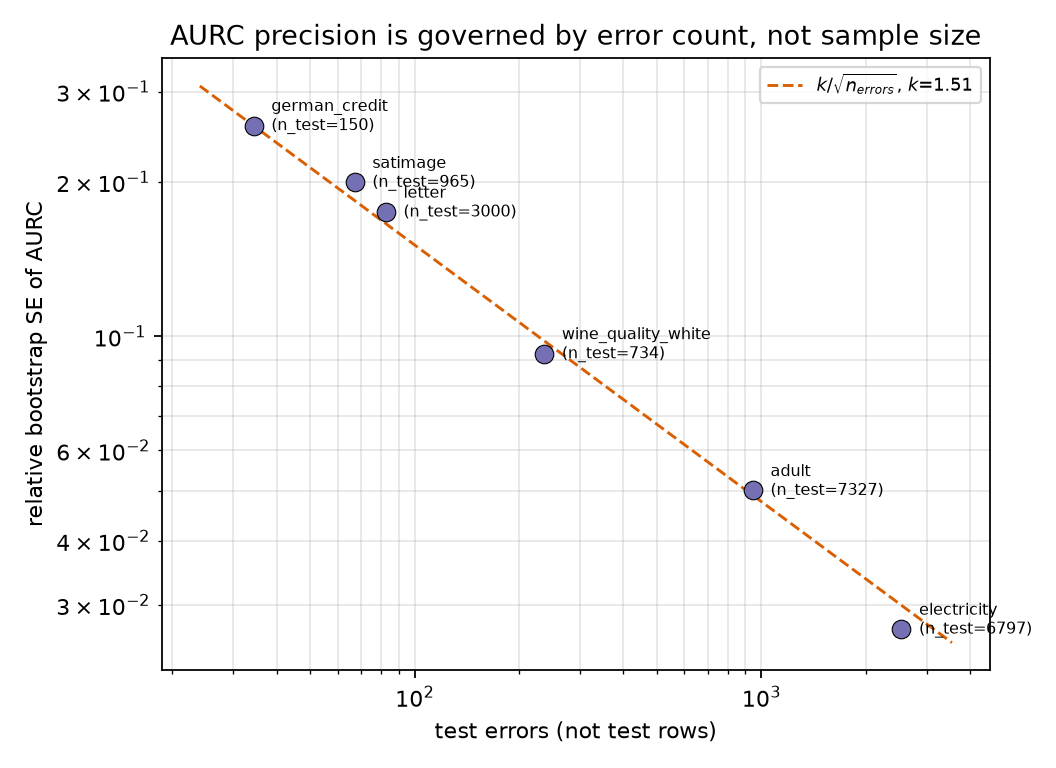
\includegraphics[width=\columnwidth]{figures/aurc_precision_vs_errors.png}
\caption{Empirical relative standard error of $\aurc$ versus test-set error count, following the binomial scaling $k/\sqrt{n_{\mathrm{err}}}$ ($k{\approx}1.51$, pooled across our six datasets, 34--2{,}533 errors). Resolving a typical 5\% improvement needs thousands of test errors.}
\label{fig:power_analysis}
\end{figure}

At 80\% power and $\alpha{=}0.05$, resolving a 5\% relative $\aurc$ difference needs ${\sim}7{,}100$ test errors in one run, or ${\sim}710$ averaged over 10 seeds -- \emph{no dataset in our registry reaches the single-run figure}. Applying a seed-averaged paired bootstrap to Table~\ref{tab:agg_vs_single}'s own three apparent wins: Letter's 95\% CI is $[-11.6,-4.5]\%$ (excludes zero) and Satimage's $[-7.1,-0.05]\%$ barely does; German Credit's $[-11.8,+0.8]\%$ does not, consistent with its win being the selection artefact identified above. Fixing the aggregator in advance changes which claims survive: only Letter remains resolvable ($[-8.1,-1.2]\%$), while Satimage's pre-registered interval ($[-4.5,+3.4]\%$) now includes zero -- the same selection effect visible in the resolvability test as in the point estimate. Of the two apparent harms, Adult is resolvable both ways; Electricity's best-of-$N$ margin actually includes zero ($[-0.4,+0.2]\%$) despite reading $-0.04\%$ on average, while its pre-registered margin is clearly resolvable ($[+2.4,+2.9]\%$) -- best-of-$N$ selection can manufacture an artificially small, noisy number even when a fixed method shows a clear effect.

\subsection{Case Study: Redundancy Is Not Shift-Invariant}
\label{sec:rq2}

$\rholocal$ describes the signal bank as fit on training-time data; it says nothing about whether that description survives deployment-time shift. We illustrate this on one dataset (Satimage, $\rholocal{\approx}0.34$ in-distribution) under controlled Gaussian covariate shift, fitting everything once on clean data.

\begin{table}[t]
\centering
\caption{Case study: Gaussian covariate shift on Satimage. Relative gap is \texttt{A1\_logreg} vs.\ best single signal; a single dataset, reported as an illustration, not a general trend.}
\label{tab:shift}
\begin{tabular}{r r l r}
\toprule
Intensity & base err.\% & Best single signal & Rel.\ gap \\
\midrule
0.00 & 6.5 & entropy & \textbf{-7.3\%} \\
0.25 & 11.2 & trust\_score & +14.6\% \\
0.50 & 17.3 & trust\_score & +32.3\% \\
2.00 & 51.6 & local\_label\_agreement & +19.0\% \\
\bottomrule
\end{tabular}
\end{table}

The aggregator wins in-distribution but its advantage reverses under shift, because Tier-C geometry overtakes MSP as the informative signal while the aggregator's weights -- frozen from clean-data fitting -- still assume MSP-like signals dominate. A diagnostic computed once at deployment time does not certify the bank's redundancy structure indefinitely; we report this as one worked example of that limitation, not as a claim about shift in general.

\subsection{Ablations}
\label{sec:ablations}

\textbf{The simplest aggregator wins.} \texttt{A1\_logreg} (plain logistic-regression stacking) is the best aggregator on Satimage, Wine, and Letter; the parameter-free rank average (A0) is best on German Credit. The neural A2 family with coverage-targeted losses never wins on any dataset -- aggregator sophistication is not what determines the outcome in Table~\ref{tab:agg_vs_single}; $\rholocal$ is.

\textbf{Ensemble disagreement never helped.} Adding five-member ensemble signals diluted gains where one existed (Wine: $-1.3\% \to -0.2\%$). Independence from MSP is necessary but not sufficient -- each added column costs the aggregator another parameter to fit from a small meta-set.

\textbf{Wine Quality: MSP is the wrong signal here, not a case of aggregation being powerful.} Against MSP, the best aggregator improves $\aurc$ by 24.5\%; but plain trust score alone attains $0.141$ versus MSP's $0.185$, and aggregation adds only a further 1.3\% on top of simply switching signals. Excluding trust score from the bank roughly doubles the aggregator's edge over the best \emph{remaining} single signal ($-1.3\% \to -2.9\%$), consistent with aggregation and single-signal substitution being partial alternatives here rather than trust score's strength being the whole explanation.

% ============================================================================
% VII. A PRACTICAL SCREENING PROTOCOL
% ============================================================================
\section{A Practical Screening Protocol}
\label{sec:protocol}

Because $\rholocal$ needs no labels, it can be computed on unlabelled held-out data \emph{before} any aggregator is trained, turning \S\ref{sec:mechanism}'s finding into a pre-deployment check rather than a post-hoc explanation.

\begin{algorithm}[t]
\caption{Boundary-Local Redundancy Screen}
\label{alg:screen}
\begin{algorithmic}[1]
\REQUIRE Frozen model $f$; unlabelled held-out set $D$; reference signal $u_{\mathrm{ref}}$ (MSP); candidate bank $\{u_1,\dots,u_m\}$; region fraction $q$ (default $0.10$)
\STATE Score $D$ with $u_{\mathrm{ref}}$ to obtain a risk ranking
\STATE $\mathcal{Q}_q \gets$ the top-$q$ fraction of $D$ by that ranking
\FOR{each $u_j$ in the bank, $j \ne \mathrm{ref}$}
  \STATE $\rho_j \gets |\rho_{\mathrm{Spearman}}(u_{\mathrm{ref}}, u_j)|$ restricted to $\mathcal{Q}_q$
\ENDFOR
\STATE $\rholocal \gets \min_j \rho_j$
\IF{$\rholocal \gtrsim 0.8$}
  \STATE \textbf{recommend:} use $u_{\mathrm{ref}}$ alone; aggregation cannot help
\ELSE
  \STATE \textbf{recommend:} aggregation may help; validate with a pre-registered aggregator on held-out seeds before deploying (\S\ref{sec:power})
\ENDIF
\end{algorithmic}
\end{algorithm}

The threshold $0.8$ is not tuned to our data: it sits well above the highest value ($0.46$) observed on any dataset where aggregation helped and well below the exact value ($1.0$) forced on every dataset where it did not, so the recommendation is robust to where exactly the line is drawn within that gap. The protocol costs one pass over held-out data and a handful of rank correlations -- orders of magnitude cheaper than training and validating an aggregator, and it never requires the labels an $\aurc$ comparison would.

% ============================================================================
% VIII. LIMITATIONS
% ============================================================================
\section{Limitations}
\label{sec:limitations}

\textbf{$\rholocal$ predicts; it is not yet shown to cause.} All three locally-redundant datasets in our benchmark are $K{=}2$, and all three others are $K{\ge}6$, so \S\ref{sec:mechanism}'s separation is confounded with class count. We attempted to break this confound in two ways, and report both honestly rather than only the one that worked. First, we screened 16 multiclass OpenML candidates for one that is simultaneously $K{\ge}3$ and locally redundant, which would decouple the two directly: none exists in a form we could evaluate -- candidates with at least 50 test errors reach at most $\rholocal{=}0.458$, and those with $\rholocal \ge 0.6$ have at most 9 test errors, because local redundancy tracks base \emph{accuracy}, which is in direct tension with having enough errors to measure anything. Second, we held $K$ fixed and swept base-model capacity instead (Fig.~\ref{fig:capacity}): binary controls confirm $\rholocal{=}1.0000$ at every capacity, exactly as the theorem requires, but on Wine Quality the resulting correlation between $\rholocal$ and aggregation gain is significant (Spearman $-0.376$, $p{=}0.041$, $n{=}30$) in the \emph{opposite} direction to our prediction, and on Satimage the capacity ladder failed to move $\rholocal$ at all. Base accuracy and effective binarity correlate with the gain more strongly than $\rholocal$ itself in this experiment, so weakening a base model appears to confound estimation difficulty with the redundancy we intended to isolate. We therefore present $\rholocal$ as an exact, causal mechanism for $K{=}2$ and a strong, unexplained empirical predictor for $K{\ge}3$ -- not yet a demonstrated cause in the latter case.

\begin{figure}[t]
\centering
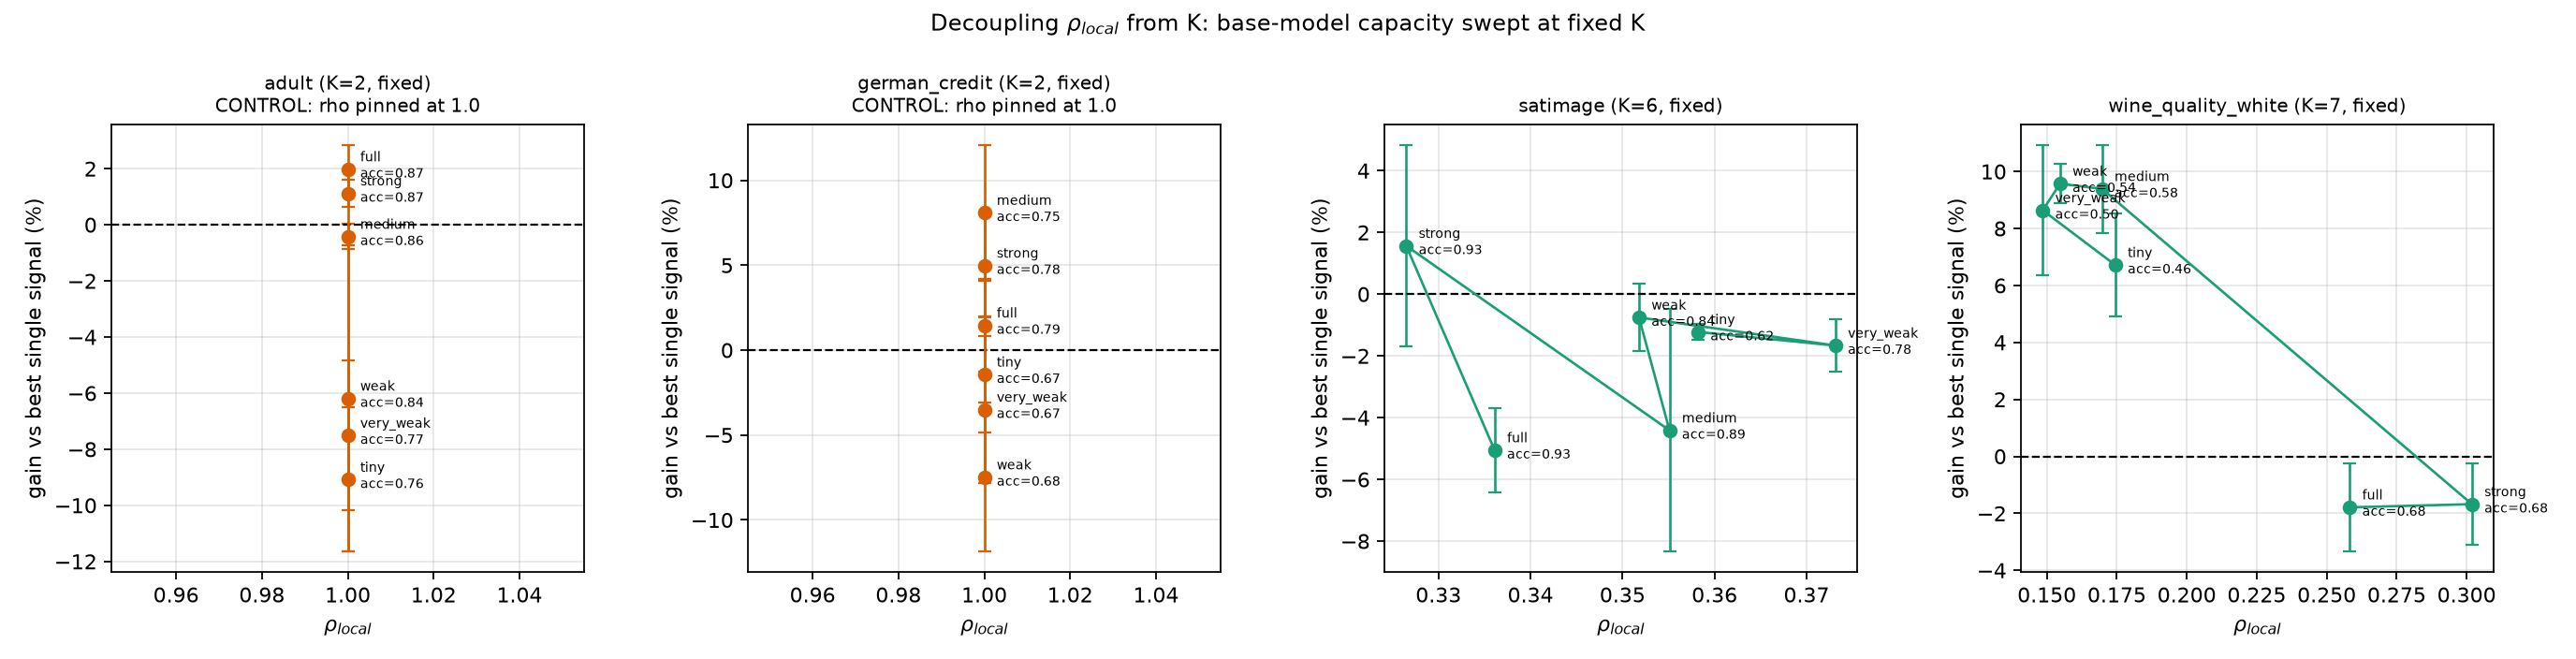
\includegraphics[width=\columnwidth]{figures/capacity_dose_response.png}
\caption{The controlled decoupling attempt: aggregation gain vs.\ $\rholocal$ as base-model capacity varies at fixed $K$. Binary controls (right) confirm $\rholocal{=}1$ at every setting; the $K{\ge}3$ panels show no dose-response (Satimage) or one running opposite to prediction (Wine Quality).}
\label{fig:capacity}
\end{figure}

\textbf{Scope.} All results are on tabular data with gradient-boosted trees; the degeneracy proof is architecture-independent, but we have not tested other model families or modalities. Only one dataset carries genuine (rather than synthetic) distribution shift, and the shift case study in \S\ref{sec:rq2} is a single worked example. Ten seeds bounds our significance tests; with Holm correction, only unanimous results reach $p{<}0.05$.

% ============================================================================
% IX. CONCLUSION
% ============================================================================
\section{Conclusion}
\label{sec:conclusion}

We asked when aggregating heterogeneous uncertainty signals can improve selective prediction over the best single signal, and answered with a mechanism rather than another benchmark entry. On binary tasks the answer is never, exactly, because the logit-derived signal family collapses to one ranking. On multiclass tasks the answer depends on redundancy measured where the risk--coverage curve is actually sensitive -- the abstention boundary, not the whole test set -- and we give a three-line, label-free protocol (Algorithm~\ref{alg:screen}) that predicts the outcome before an aggregator is ever trained, with perfect separation across six benchmark datasets. We are equally explicit about what this protocol has not yet earned: a demonstrated causal role at fixed class count, which our own controlled experiment did not establish and in one case contradicted. The practical rule that survives all of this: before building a multi-signal aggregation pipeline, check whether the bank induces different rankings where it matters, because plausible-sounding diversity is not sufficient, and the check is far cheaper than the pipeline.

% ============================================================================
% REFERENCES
% ============================================================================
\bibliographystyle{IEEEtran}
\bibliography{references}

\end{document}
